\documentclass[12pt]{article}
\usepackage[utf8]{inputenc}
\usepackage{amsmath, amssymb}
\usepackage{hyperref}
\usepackage{tikz}
\usepackage[left=2.5cm,right=2.5cm,bottom=2.5cm]{geometry}

\hypersetup{
    colorlinks=true}

\title{MATH 5707 (Spring 2026): Homework 3}
\date{}

\begin{document}
\vspace{-0.7in}

\maketitle
\vspace{-0.6in}

\section*{Directions and Introduction}
Submit a pdf of your solutions to the HW 3 assignment on Gradescope by 11:59 pm on February 20.

Problem 2 is marked as a peer review problem. \href{https://docs.google.com/document/d/1jSw9pmMJJFUx_6dTkcUi4k4HJNIrrIIgs9zdWhAycx0/edit?usp=sharing}{This document gives directions and deadlines for the peer review process.}

When working on this assignment, you should focus on showing fluency with the following skills:
\begin{itemize}
    \item Clearly communicate solutions using complete sentences and enough explanation that another 5707 student could follow your work.
    \item Demonstrate fluency with the concept of trees.
   \item Write proofs involving trees. 
    \item Determine whether or not a given statement is true.
    \item Write a clear disproof of a false statement using an example. 
    \item Translate a scenario or problem into a question or statement about graphs.
\end{itemize}


\section*{Problems}

\begin{enumerate}
\item[0.] If you would like any of these problems to be graded for proficiency with the core skills, list the skill and the corresponding problem. 
  \item Consider the graph $G$ below.
  
  \begin{center}
    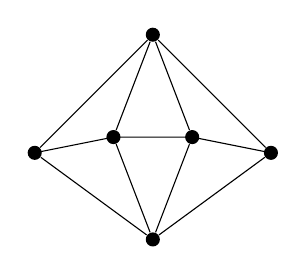
\begin{tikzpicture}
    \draw[every node/.style={inner sep=1.8pt,fill,circle}]
    (-1.5,-.2)node(x1){}--(-.5,0)node(x2){}--(.5,0)node(x3){}--(1.5,-.2)node(x4){};
    \draw[every node/.style={inner sep=1.8pt,fill,circle}]
    (0,1.3)node(a){} (0,-1.3)node(b){}
    \foreach \x in {1,2,3,4}{
    (a)--(x\x)--(b)};
    \end{tikzpicture}
  \end{center}
  
  \begin{enumerate}
  \item Find all of the spanning trees of $G$.  Draw them all.
  \item How many non-isomorphic spanning trees does $G$ have? Justify your answer by explaining why pairs of trees from part (a) are or are not isomorphic. 
  \end{enumerate}
    \item  (2.1.12 from Bondy-Murty, peer review problem) A saturated hydrocarbon is a molecule $C_mH_n$ in which every carbon atom has four bonds, every hydrogen atom has one bond, and no sequence of bonds forms a cycle.  Show that, for every positive integer $m$, $C_mH_n$ can exist only if $n=2m+2$. 

  \item Prove or disprove the following statements. (Each part will be worth 4 points and graded as a separate problem.)
  \begin{enumerate}
  \item If $G$ is a tree with maximum degree at least $k$, then $G$ has at least $k$ leaves. 
  \item Any simple graph with $n$ vertices and $n-1$ edges must be a tree. 
  \item If $T_1$ and $T_2$ are two trees with the same degree sequence, then $T_1\cong T_2$.
  \end{enumerate}


\end{enumerate}

\end{document}
